\section{Architecture Integration}

\subsection{Model Support}

\begin{table}[H]
\centering
\small
\begin{tabular}{llllll}
\toprule
\textbf{Model} & \textbf{Attention} & \textbf{Nested?} & \textbf{RoPE?} & \textbf{GQA?} & \textbf{Cross-attn} \\
\midrule
DistilBERT & \texttt{layer[i].attention} & No & No & No & No \\
RoBERTa & \texttt{layer[i].attention.self} & Yes & No & No & No \\
GPT-2 & \texttt{h[i].attn} & No & No & No & No \\
Qwen3.5 & \texttt{layers[i].self\_attn} & No & Yes & Yes & No \\
T5 & \texttt{block[i].layer[0]} & No & No & No & Yes \\
\bottomrule
\end{tabular}
\end{table}

\subsection{Weight Extraction Patterns}

\subsubsection{GPT-2 Conv1D}

\begin{lstlisting}
c\_w = c\_attn.weight.t()
q\_w, k\_w, v\_w = c\_w.chunk(3, dim=0)
o\_w = c\_proj.weight.t()
\end{lstlisting}

\subsubsection{RoBERTa Nested}

\begin{lstlisting}
q\_w = src.self.query.weight
k\_w = src.self.key.weight
v\_w = src.self.value.weight
o\_w = src.output.dense.weight
\end{lstlisting}

\subsubsection{Flat Modules}

Direct attribute access on \texttt{q\_lin} / \texttt{q\_proj} / \texttt{query}.

\subsubsection{UniversalAdapter Fallback}

If any projection is missing.

\subsection{Handling of the MoE Dimension}

The MoE operates on \texttt{all\_head\_size = num\_heads * head\_dim}. This equals the 
hidden dimension for standard attention.

\textbf{For GQA models}, \texttt{kv\_head\_size \textless{} all\_head\_size}. But the attention output 
is always \texttt{all\_head\_size} (Q heads $\times$ head dim). So the MoE input dimension 
is always \texttt{all\_head\_size = d}.

\subsection{Dynamic Dimension Adaptation}

If the incoming hidden size differs from the router's input size, a 
\textbf{dynamic router} is created on-the-fly:

\begin{lstlisting}
if D == self.d\_model:
    logits = self.router(self.router\_ln(x\_flat))
else:
    normed = F.layer\_norm(x\_flat, (D,))
    if not hasattr(self, "\_dynamic\_router") or self.\_dynamic\_router.in\_features != D:
        self.\_dynamic\_router = nn.Linear(D, self.n\_experts, bias=False)...
    logits = self.\_dynamic\_router(normed)
\end{lstlisting}

This handles cross-attention where the input dimension may differ.

\subsection{Nested Encoder Bypass}

For RoBERTa, \texttt{is\_nested\_encoder = True}:

\begin{lstlisting}
if self.is\_nested\_encoder:
    if enriched\_attn.shape[-1] != self.dim:
        out = self.out\_lin(enriched\_attn)
    else:
        out = enriched\_attn
\end{lstlisting}

The outer \texttt{attention.output.dense} handles the projection.

\subsection{Causality}

For decoders, causal masking is applied to attention scores:

\begin{lstlisting}
if self.is\_decoder and not is\_cross\_attention:
    causal\_mask = torch.triu(torch.full((L, kv\_len), -inf, ...), diagonal=1)
    scores = scores + causal\_mask.unsqueeze(0).unsqueeze(1)
\end{lstlisting}

The MoE operates on the attention output, which is already causal.

\subsection{Injection Algorithm}

\textbf{Algorithm 2:} Inject ExpertChoiceMoEAttention
\begin{lstlisting}
Input:  model M, config c, n\_experts, capacity\_factor
Output: M with attention replaced

1: for each layer:
2:     src $\leftarrow$ extract\_attention(layer)
3:     if src is None: continue
4:     try:
5:         new $\leftarrow$ ExpertChoiceMoEAttention(c, n\_experts=E, ...)
6:         replace(layer, new)
7:     except Exception:
8:         raise RuntimeError("copy\_weights failed")
9: return M
\end{lstlisting}

\subsection{Failure Handling}

The injection raises \texttt{RuntimeError} on any failure. This is strict because 
MoE injection is complex.

\subsection{Registry}

\begin{lstlisting}
@ATTENTION\_REGISTRY.register("expert\_choice\_moe")
@ATTENTION\_REGISTRY.register("expert\_choice\_moe\_attention")
class ExpertChoiceMoEAttention(BaseAttention):
    ...
\end{lstlisting}



\begin{figure}[H]
\centering
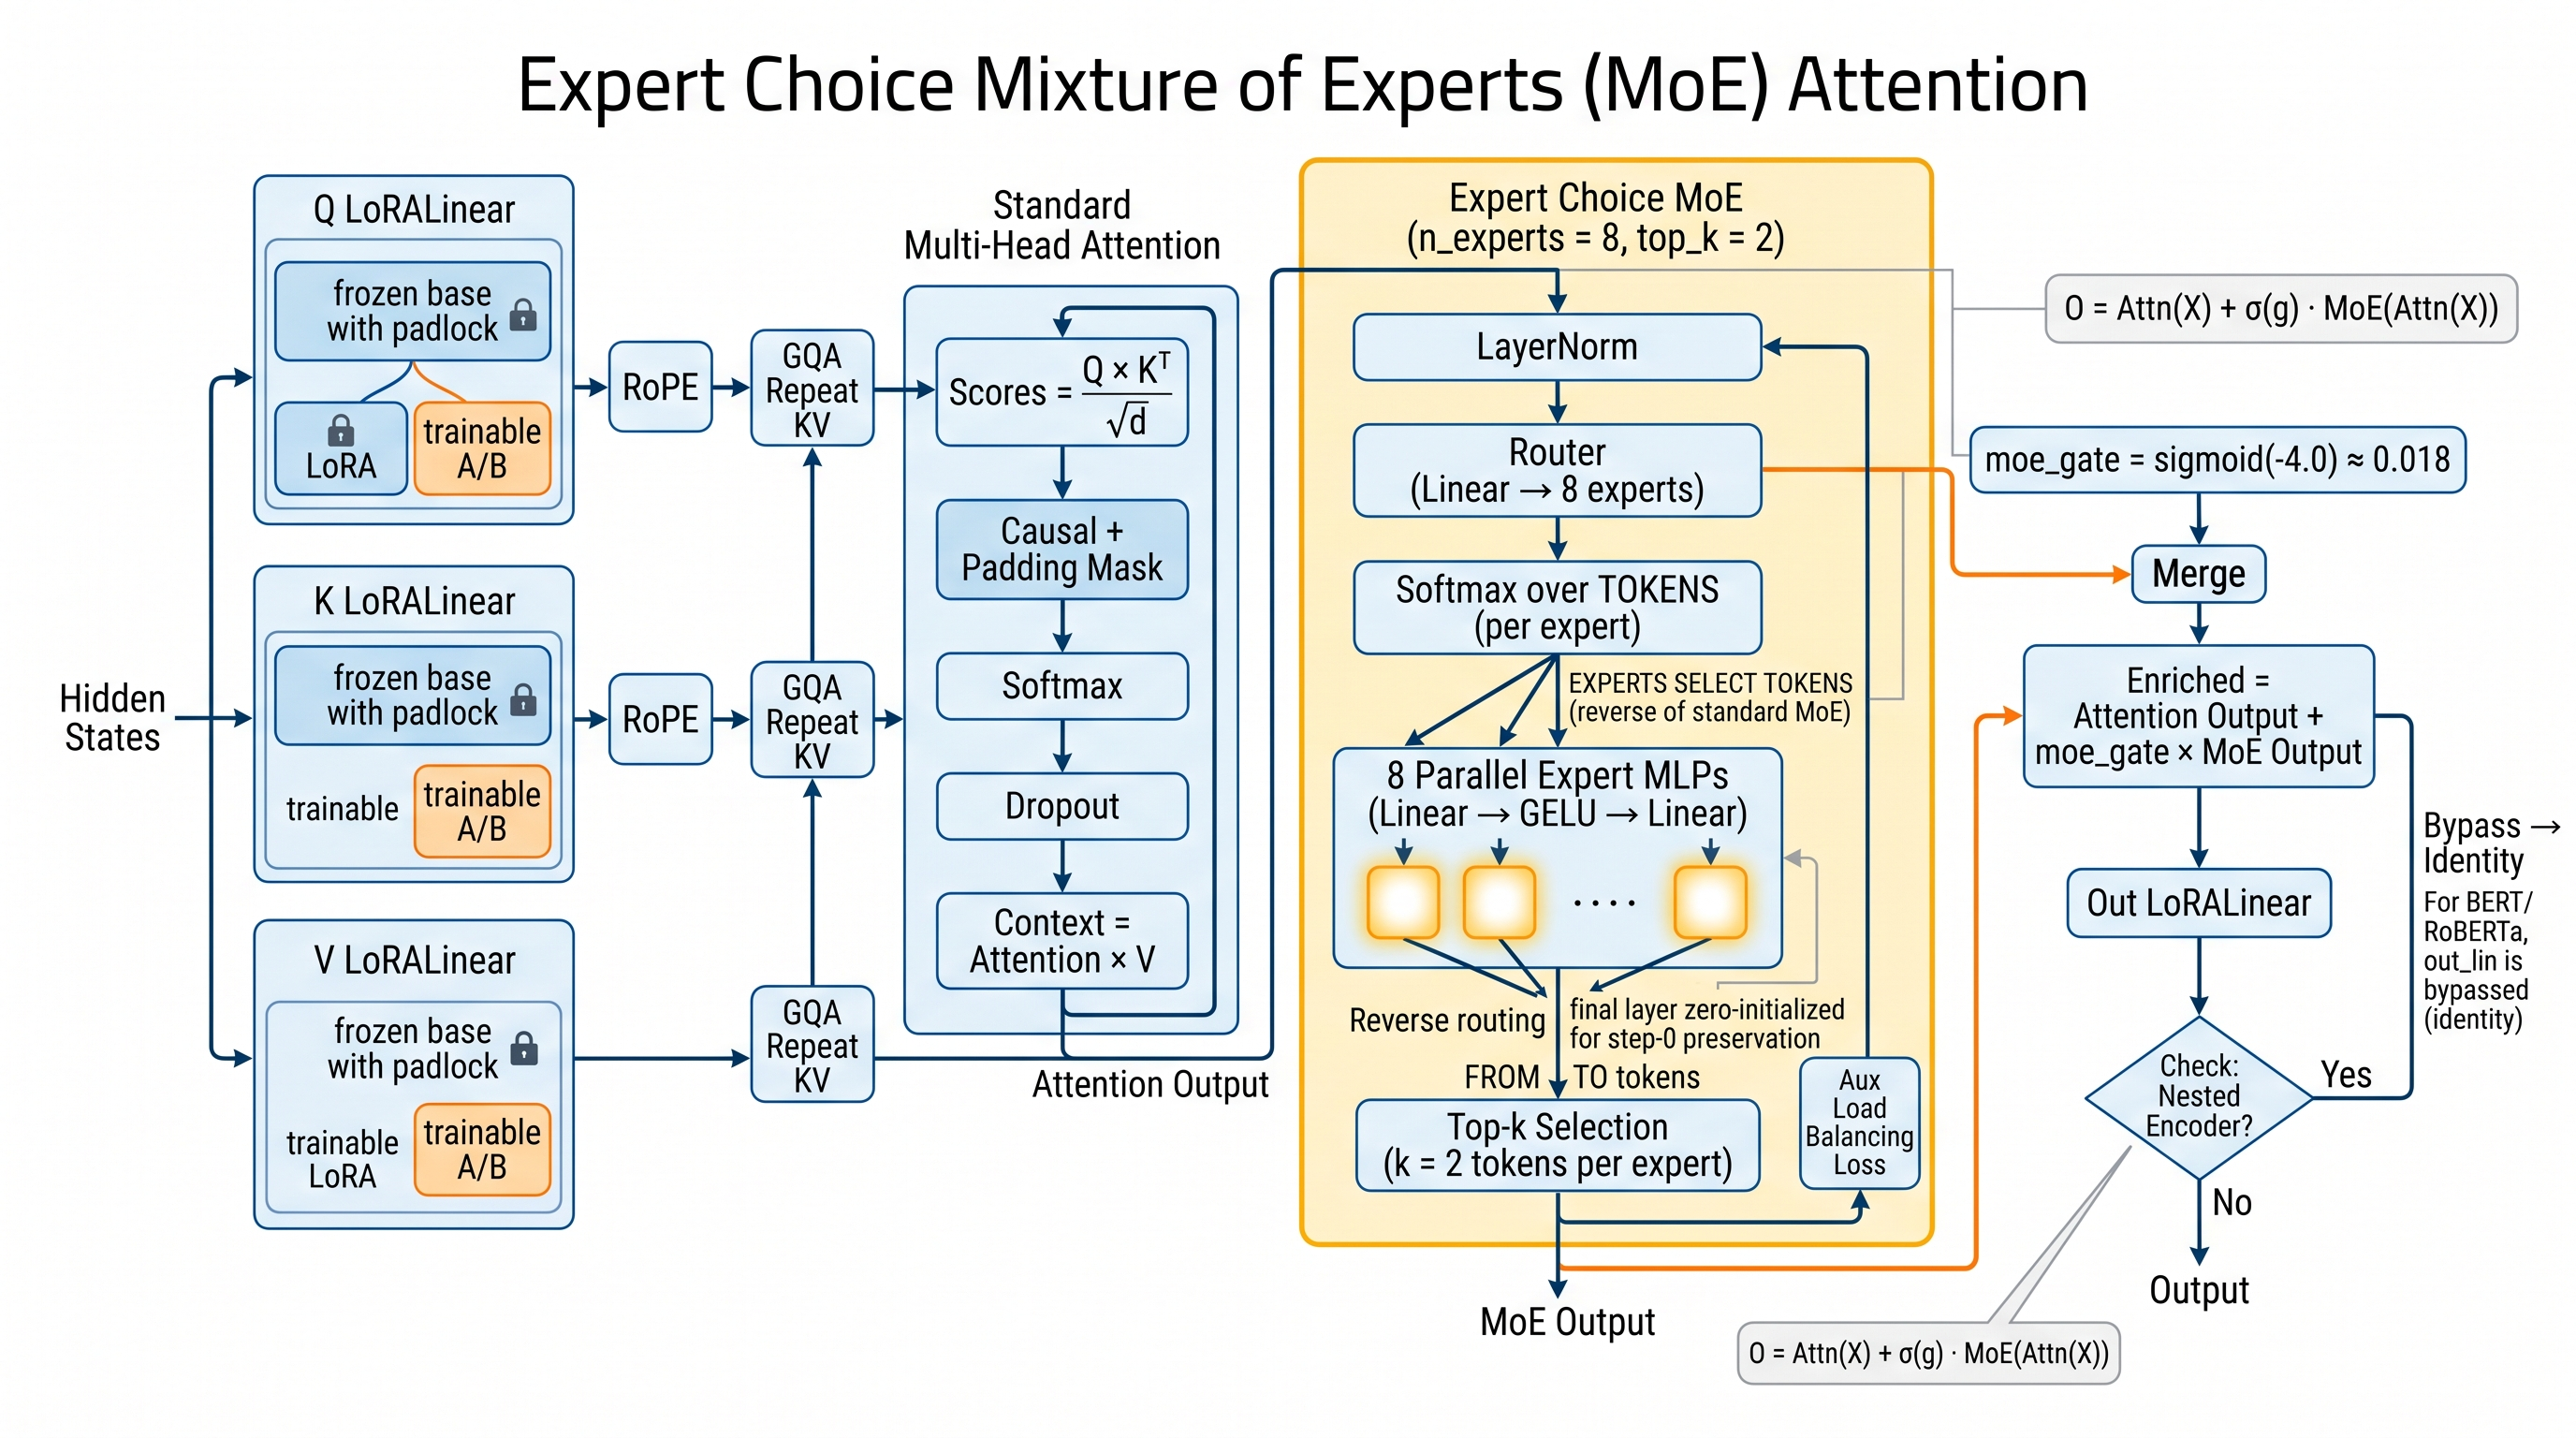
\includegraphics[width=\linewidth]{figures/architecture.jpeg}
\caption{High-level architectural diagram of expert\_choice\_moe.}
\label{fig:arch_expert-choice-moe}
\end{figure}

